\chapter{Dodatna vaja}
\section{Realizacija preprostega procesorja}

Z gradniki, ki smo jih spoznali, se bomo lotili izdelave preprostega procesorja. Procesor je hipotetičen in izjemno poenostavljen, v osnovi pa je njegovo delovanje vseeno enako, kot delovanje kompleksnejših procesorjev. 

\section{Osnovno delovanje procesorja}
Predpostavljamo, da naš procesor vsak ukaz izvrši v dveh urinih periodah. Procesor torej deluje v dveh stopnjah, in sicer:
\begin{itemize}
\item \emph{prevzem ukaza} \angl{Instruction Fetch, IF},
\item \emph{izvedba ukaza} \angl{Execute, EX}.
\end{itemize}

V nadaljevanju je opisana posamezna stopnja. Procesor lahko postavimo v začetno stanje (t.j. prevzem ukaza) z \emph{Reset} vhodom.

\subsection{Prevzem ukaza}
V prvi urini periodi se iz pomnilnika, ki vsebuje sekvenco ukazov, t.i. \emph{ukaznega pomnilnika}, prebere ukaz. Pomnilnik vsebuje več ukazov, pri čemer se vsak ukaz nahaja na svojem naslovu. Naslov iz katerega se bere trenutni ukaz je shranjen v registru, ki ga imenujemo \emph{programski števec} \angl{Program Counter}. Prebrani ukaz se shrani v \emph{ukazni register} \angl{Instruction Register}, kjer počaka na izvedbo, ki se izvrši v naslednji urini periodi - v stopnji \emph{izvedba ukaza}. 

Ko je ukaz zapisan v ukazni register, se lahko programski števec poveča. S tem dosežemo, da bo v naslednji stopnji, t.j. \emph{prevzem ukaza}, prevzet naslednji ukaz iz ukaznega pomnilnika. Zaporedje ukazov v ukaznem pomnilniku tako sestavlja \emph{program}, ki ga naš procesor izvaja.

\subsection{Izvedba ukaza}
Stopnja \emph{izvedba ukaza} izvede ukaz, ki je zapisan v ukaznem registru. Pri našem procesorju je to lahko branje ali pisanje v pomnilnik ali aritmetično-logični operaciji: seštevanje in odštevanje. 

Izvedba ukaza se izvrši tako, da kontrolna enota ukaz, ki je zapisan v ukaznem registru najprej \emph{dekodira} (posamezen ukaz ima svojo kodo, ki je enolično določena s sekvenco bitov). V skladu z dekodiranim ukazom kontrolna enota določi vrednosti t.i. \emph{kontrolnih signalov}, ki služijo kot vhodi v ostale komponente, ki opravijo dejansko izvedbo ukaza. 

V našem primeru lahko kontrolno enoto predstavimo z Mealyjevim avtomatom z dvema stanjema in sedmimi različnimi prehodi med njima (glej Sliko \ref{fig:CU}). Avtomat v vsaki urini periodi preide iz stanja IF v stanje EX (razen v primeru aktivnosti vhoda $Reset$). Medtem, ko je iz stanja IF v stanje EX možen le en prehod (prevzem ukaza), lahko prehod iz stanja EX v stanje IF kontrolna enota izvede preko petih prehodov -- izbira prehoda je odvisna od ukaza, ki ga je procesor prevzel pri prehodu kontrolne enote iz stanja IF v stanje EX. 

\section{Osnovna arhitektura procesorja}
Procesor je v našem primeru sestavljen iz sledečih komponent:
\begin{itemize}
\item splošno namenski registri ($A$ in $B$),
\item programski števec \angl{Program Counter, PC},
\item ukazni register \angl{Instruction Register, IR},
\item kontrolna enota \angl{Control Unit, CU},
\item aritmetično logična enota \angl{Arithmetic Logic Unit, ALU},
\item ukazni pomnilnik \angl{Instruction Memory, IM},
\item podatkovni pomnilnik \angl{Data Memory, DM},
\item ostala kombinatorna logika.
\end{itemize}
Posamezna komponenta je podrobneje opisana v nadaljevanju.

\subsection{Splošno namenski registri}
Aritmetično logična enota izvaja aritmetično logične operacije (oziroma v našem primeru zgolj aritmetične operacije) nad podatki, ki so shranjeni v pomnilniku. Rezultati teh operacij se morajo slej ko prej zapisati nazaj v pomnilnik. Splošno namenski registri služijo kot vmesnik med pomnilnikom in aritmetično logično enoto, saj aritmetično logična enota ne more neposredno dostopati do podatkov zapisanih v pomnilniku. Splošno namenski registri se torej uporabljajo za shranjevanje vmesnih rezultatov aritmetično logičnih operacij.

V našem primeru bomo imeli 2 2-bitna splošno namenska registra. Imenujemo ju register A in register B. Aritmetične operacije (seštevanje in odštevanje) lahko torej delamo nad dvema 2-bitnima podatkoma.

\subsection{Programski števec}
V stopnji \emph{prevzem ukaza} se iz ukaznega pomnilnika prebere ukaz. Ukaz se zatem shrani v \emph{ukazni register}. Pomnilniški naslov iz katerega se prebere ukaz, je zapisan v registru, ki mu rečemo \emph{programski števec}. 

V našem primeru je programski števec 2-bitni register. Naslavljamo lahko torej 4 pomnilniške lokacije - maksimalna dolžina programa v ukaznem pomnilniku so 4 ukazi.

\subsection{Ukazni register}
V \emph{ukazni register} se shrani ukaz, ki je bil prebran iz ukaznega pomnilnika v stopnjo \emph{prevzem ukaza}. Na podlagi vsebine ukaznega registra v stopnji \emph{izvedba ukaza} kontrolna enota določi vrednosti kontrolnih signalov. Kontrolni signali služijo kot vhodi v ostale komponente, ki opravijo dejansko izvedbo ukaza.

V našem primeru je ukazni register 4-bitni register. Naš procesor torej podpira 4-bitne ukaze. 

\subsection{Kontrolna enota}
Kontrolna enota skrbi za izvedbo prevzema naslednjega ukaza in njegovo izvedbo. V skladu s trenutno stopnjo izvedbe ukaza in trenutnim ukazom določi vrednosti kontrolnih signalov, ki služijo kot vhodi v ostale komponente, ki opravijo dejanski prevzem in izvedbo ukaza. Kontrolno enoto lahko predstavimo z Mealyjevim avtomatom z dvema stanjema in sedmimi različnimi prehodi med njima (glej Sliko \ref{fig:CU}). 

%\begin{figure}%
%\begin{center}
%\begin{tikzpicture}[scale=0.2]
%\tikzstyle{every node}+=[inner sep=0pt]
%\draw [black] (67,-25.7) circle (3);
%\draw (67,-25.7) node {$EX$};
%\draw [black] (16.2,-25.7) circle (3);
%\draw (16.2,-25.7) node {$IF$};
%\draw [black] (10.1,-22.1) -- (13.62,-24.18);
%\draw (9.45,-20.85) node [left] {$Reset/-$};
%\fill [black] (13.62,-24.18) -- (13.18,-23.34) -- (12.67,-24.2);
%\draw [black] (17.821,-23.177) arc (144.34749:35.65251:29.264);
%\fill [black] (65.38,-23.18) -- (65.32,-22.24) -- (64.51,-22.82);
%\draw (41.6,-10.47) node [above] {$-/IR\leftarrow IM[PC];\mbox{ }PC\leftarrow PC+1$};
%\draw [black] (19.136,-25.084) arc (101.1181:78.8819:116.496);
%\fill [black] (19.14,-25.08) -- (20.02,-25.42) -- (19.82,-24.44);
%\draw (41.6,-22.4) node [above] {$LOAD\mbox{ }A/A\leftarrow DM[IR[1..0]]$};
%\draw [black] (64.042,-26.2) arc (-81.00822:-98.99178:143.589);
%\fill [black] (19.16,-26.2) -- (19.87,-26.82) -- (20.03,-25.83);
%\draw (41.6,-28.46) node [below] {$LOAD\mbox{ }B/B\leftarrow DM[IR[1..0]]$};
%\draw [black] (64.662,-27.579) arc (-53.42302:-126.57698:38.702);
%\fill [black] (18.54,-27.58) -- (18.88,-28.46) -- (19.48,-27.65);
%\draw (41.6,-35.7) node [below] {$STORE\mbox{ }A/DM[IR[1..0]]\leftarrow A$};
%\draw [black] (66.579,-28.669) arc (-11.44783:-168.55217:25.486);
%\fill [black] (16.62,-28.67) -- (16.29,-29.55) -- (17.27,-29.35);
%\draw (41.6,-49.6) node [below] {$SUB/A\leftarrow A-B$};
%\draw [black] (65.543,-28.321) arc (-32.10627:-147.89373:28.266);
%\fill [black] (17.66,-28.32) -- (17.66,-29.26) -- (18.51,-28.73);
%\draw (41.6,-42.06) node [below] {$ADD/A\leftarrow A+B$};
%\end{tikzpicture}
%\end{center}
%\caption{Mealyjev avtomat kontrolne enote procesorja.}%
%\label{fig:CU}%
%\end{figure}

\begin{figure}%
\begin{center}
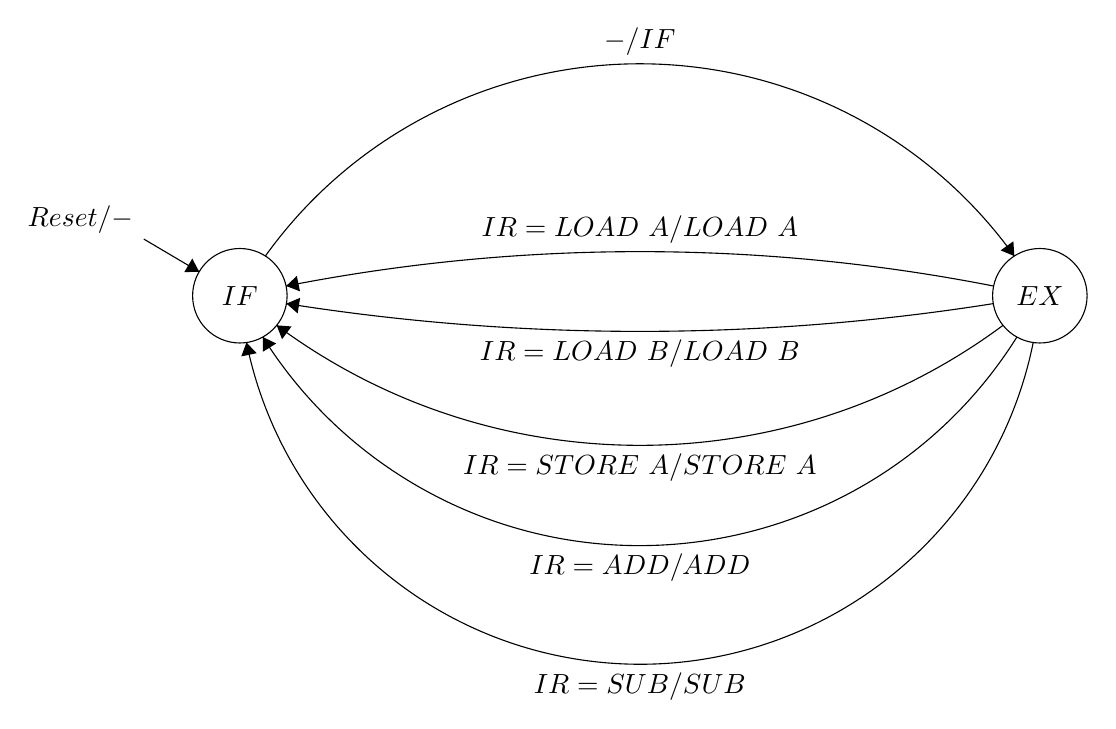
\begin{tikzpicture}[scale=0.2]
\tikzstyle{every node}+=[inner sep=0pt]
\draw [black] (67,-25.7) circle (3);
\draw (67,-25.7) node {$EX$};
\draw [black] (16.2,-25.7) circle (3);
\draw (16.2,-25.7) node {$IF$};
\draw [black] (10.1,-22.1) -- (13.62,-24.18);
\draw (9.45,-20.85) node [left] {$Reset/-$};
\fill [black] (13.62,-24.18) -- (13.18,-23.34) -- (12.67,-24.2);
\draw [black] (17.821,-23.177) arc (144.34749:35.65251:29.264);
\fill [black] (65.38,-23.18) -- (65.32,-22.24) -- (64.51,-22.82);
\draw (41.6,-10.47) node [above] {$-/IF$};
\draw [black] (19.136,-25.084) arc (101.1181:78.8819:116.496);
\fill [black] (19.14,-25.08) -- (20.02,-25.42) -- (19.82,-24.44);
\draw (41.6,-22.4) node [above] {$IR = LOAD\mbox{ }A/LOAD\mbox{ }A$};
\draw [black] (64.042,-26.2) arc (-81.00822:-98.99178:143.589);
\fill [black] (19.16,-26.2) -- (19.87,-26.82) -- (20.03,-25.83);
\draw (41.6,-28.46) node [below] {$IR = LOAD\mbox{ }B/LOAD\mbox{ }B$};
\draw [black] (64.662,-27.579) arc (-53.42302:-126.57698:38.702);
\fill [black] (18.54,-27.58) -- (18.88,-28.46) -- (19.48,-27.65);
\draw (41.6,-35.7) node [below] {$IR = STORE\mbox{ }A/STORE\mbox{ }A$};
\draw [black] (66.579,-28.669) arc (-11.44783:-168.55217:25.486);
\fill [black] (16.62,-28.67) -- (16.29,-29.55) -- (17.27,-29.35);
\draw (41.6,-49.6) node [below] {$IR = SUB/SUB$};
\draw [black] (65.543,-28.321) arc (-32.10627:-147.89373:28.266);
\fill [black] (17.66,-28.32) -- (17.66,-29.26) -- (18.51,-28.73);
\draw (41.6,-42.06) node [below] {$IR = ADD/ADD$};
\end{tikzpicture}
\end{center}
\caption{Mealyjev avtomat kontrolne enote procesorja.}%
\label{fig:CU}%
\end{figure}

Kontrolna enota ima torej dve stanji, tj. stanje \emph{IF}, ki je aktivno, ko je procesor v stopnji \emph{prevzem ukaza} in stanje \emph{EX}, ki je aktivno, ko je procesor v stopnji \emph{izvedba ukaza}. Kot vhodne črke procesor sprejema \emph{Reset} vhod in vsebino ukaznega registra (IR). Kontrolna enota določa vrednosti izhodnih signalov, ki so hkrati njene izhodne črke, na sledeč način:
\begin{itemize}
\item \emph{IF}: izhodna črka je aktivna pri prehodu iz stanja \emph{IF} v stanje \emph{EX}. V tem primeru kontrolna enota sproži nalaganje naslednjega ukaza v ukazni register ($IR\leftarrow IM[PC]$) in povečanje vrednosti programskega števca ($PC\leftarrow PC+1$).
\item \emph{LOAD A}: izhodna črka je aktivna pri prehodu iz stanja \emph{EX} v stanje \emph{IF} pri pogoju, da je v ukaznem registru ukaz \emph{LOAD A}. V tem primeru kontrolna enota sproži nalaganje podatka iz podatkovnega pomnilnika (DM) v register $A$. Pri tem je pomnilniški naslov določen s spodnjima bitoma ukaznega pomnilnika ($A\leftarrow DM[IR[1..0]]$).
\item \emph{LOAD B}: izhodna črka je aktivna pri prehodu iz stanja \emph{EX} v stanje \emph{IF} pri pogoju, da je v ukaznem registru ukaz \emph{LOAD B}. V tem primeru kontrolna enota sproži nalaganje podatka iz podatkovnega pomnilnika (DM) v register $B$. Pri tem je pomnilniški naslov določen s spodnjima bitoma ukaznega pomnilnika ($B\leftarrow DM[IR[1..0]]$).
\item \emph{STORE A}: izhodna črka je aktivna pri prehodu iz stanja \emph{EX} v stanje \emph{IF} pri pogoju, da je v ukaznem registru ukaz \emph{STORE A}. V tem primeru kontrolna enota sproži nalaganje vsebine registra $A$ v podatkovni pomnilnik (DM), in sicer na naslov, ki je določen s spodnjima bitoma ukaznega pomnilnika ($DM[IR[1..0]]\leftarrow A$).
\item \emph{ADD}: izhodna črka je aktivna pri prehodu iz stanja \emph{EX} v stanje \emph{IF} pri pogoju, da je v ukaznem registru ukaz \emph{ADD}. V tem primeru kontrolna enota sproži seštevanje vsebine registra $A$ in vsebine registra $B$, pri čemer se rezultat shrani v register $A$ ($A\leftarrow A+B$).
\item \emph{SUB}: izhodna črka je aktivna pri prehodu iz stanja \emph{EX} v stanje \emph{IF} pri pogoju, da je v ukaznem registru ukaz \emph{SUB}. V tem primeru kontrolna enota sproži odštevanje vsebine registra $B$ od vsebine registra $A$, pri čemer se rezultat shrani v register $A$ ($A\leftarrow A-B$).
\end{itemize}


Realizacijo avtomata kontrolne enote v Logisimu prikazuje slika \ref{fig:CU_logisim}.

\begin{figure}
\begin{center}
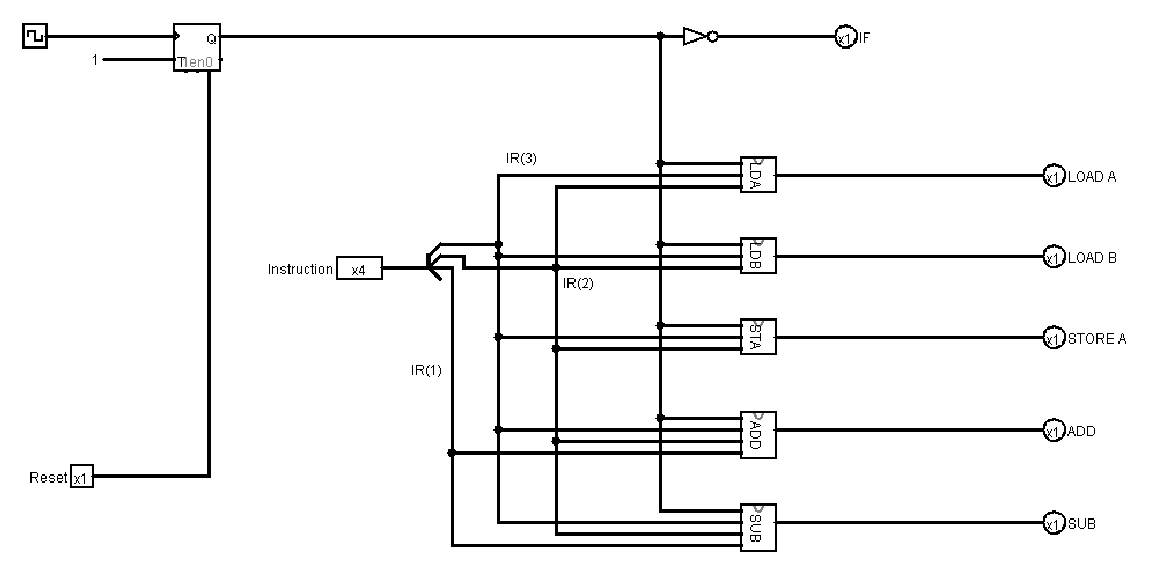
\includegraphics[width=0.75\columnwidth]{procesor/img/CU}%
\caption{Realizacija kontrolne enote v Logisimu s T-pomnilno celico, pri čemer moduli $LDA$, $LDB$, $STA$, $ADD$ in $SUB$ predstavljajo kombinatorno logiko za določitev posameznega kontrolnega signala, $Instruction$ pa ukaz, zapisan v ukaznem registru. Simbol, ki se v shemi nahaja pred komponento $Instruction$, predstavlja komponento, ki več enobitnih signalov združi v večbitni vektor.}%
\label{fig:CU_logisim}%
\end{center}
\end{figure}



\subsection{Aritmetično logična enota}
Aritmetično logična enota \angl{Arithmetic Logic Unit, ALU} izvaja aritmetično logične operacije nad splošno namenskimi registri kot so seštevanje, množenje, deljenje, logični pomik itd. V našem primeru ALU podpira samo dve artimetični operaciji, in sicer seštevanje in odštevanje vsebine registrov A in B. Operacija, ki se bo izvedla, je določena s kontrolnim signalom, katerega vrednost na podlagi dekodiranega signala določi kontrolna enota. Realizacija ALU v Logisimu je prikazana na sliki \ref{fig:ALU}, pri čemer sta vhoda $A$ in $B$ izhoda iz splošno namenskih registrov, vhod $SUB$ pa izhod iz kontrolne enote, ki ima vrednost 1, če je trenutni ukaz odštevanje. Izhod iz aritmetično logične enote določa rezultat izvedene operacije.

\begin{figure}
\begin{center}
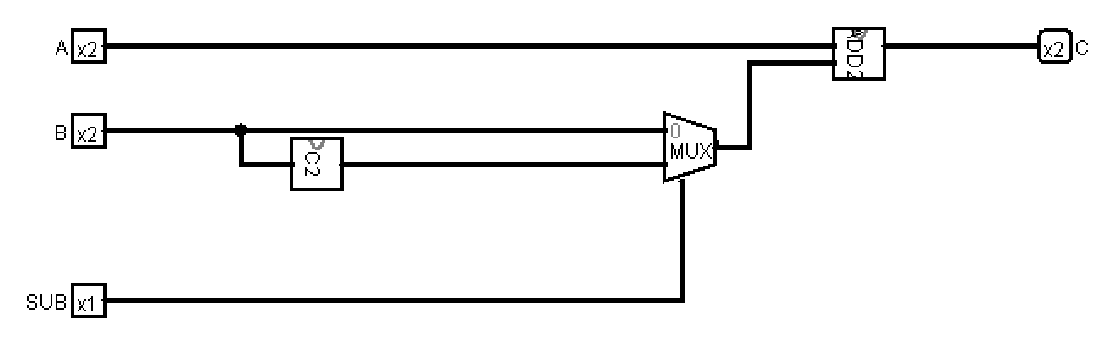
\includegraphics[width=0.75\columnwidth]{procesor/img/ALU}%
\caption{Realizacija aritmetično logične enote v Logisimu, pri čemer $ADD2$ predstavlja modul za izračun vsote 2-bitnih vhodov, $C2$ pa modul za izračun dvojiškega komplementa 2-bitnega vhoda (glej razdelek \ref{sec:odstevalnik}). Naslovni vhod v multiplekser ($SUB$) določi ali se bo izračunala vsota števil $A$ in $B$ ali vsota števila $A$ in dvojiškega komplementa števila $B$.}%
\label{fig:ALU}%
\end{center}
\end{figure}

\subsection{Ukazni pomnilnik}
V ukaznem pomnilniku so shranjeni ukazi za izvedbo. Na podlagi podanega naslova se iz ukaznega pomnilnika prebere ukaz za izvedbo. Na sekvenco ukazov v ukaznem pomnilniku lahko tako gledamo kot na program, ki ga bo naš procesor izvajal.

V našem primeru je ukazni pomnilnik realiziran z ROM pomnilnikom, v katerega zapišemo program pred zagonom procesorja. Na voljo imamo 4 lokacije (program je lahko dolg 4 ukaze). Pomnilnik torej naslavljamo z 2-bitnim naslovom. Ukazi v pomnilniku so dolgi 4 bite. 

\subsection{Podatkovni pomnilnik}
Podatkovni pomnilnik vsebuje podatke nad katerimi procesor izvaja aritmetično logične operacije. Branje iz podatkovnega pomnilnika poteka preko registrov A in B. V pomnilnik lahko zapisujemo zgolj preko registra A. Prav tako kot pri ukaznem pomnilniku, tudi pri podatkovnem pomnilniku vedno podajamo naslov na katerega zapisujemo podatek oziroma s katerega beremo. V podatkovni pomnilnik lahko shranimo 4 podatke velikosti 2 bita. Naslavljamo ga torej z 2-bitnim naslovom.

\subsection{Ostala kombinatorna logika}
To so multiplekserji in ostala kombinatorna logična vrata.

\section{Nabor ukazov}
Procesor podpira izvedbo 5 različnih ukazov (glej Tabelo \ref{tab:ukazi}). Posamezen ukaz je določen s 4-bitno kodo, ki je shranjena v ukaznem pomnilniku oziroma ukaznem registru. Pri nekaterih ukazih se del te kode uporabi kot naslov za podatkovni pomnilnik. 

\begin{table}
\begin{tabular}{cccc|c|c}
 $IR(3)$ & $IR(2)$ & $IR(1)$ & $IR(0)$ & ukaz & pomen \\
 \hline
 $0$ & $0$ & $x$ & $y$ &  $Load\ A\ DM[(x,y)]$ & $A \leftarrow DM[(x,y)]$\\		 
 $0$ & $1$ & $x$ & $y$ &  $Load\ B\ DM[(x,y)]$ & $B \leftarrow DM[(x,y)]$\\		  
 $1$ & $0$ & $x$ & $y$ &  $Store\ A\ DM[(x,y)]$ & $DM[(x,y)] \leftarrow A$\\		 
 $1$ & $1$ & $0$ & $?$ &  $Add$ & $A \leftarrow A + B$\\
 $1$ & $1$ & $1$ & $?$ &  $Sub$ & $A \leftarrow A - B$\\		 
\end{tabular}
\caption{Seznam in pomen ukazov, ki jih podpira naš procesor. Pri tem $DM[(x,y)]$ predstavlja lokacijo v podatkovnem pomnilniku na 2-bitnem naslovu $(x,y)$.}
\label{tab:ukazi}
\end{table}

V nadaljevanju so ukazi podrobneje opisani.

\subsection{Load A}

Ukaz \emph{Load A} v register A naloži vrednost iz pomnilniškega naslova, ki je določen z bitoma $IR(1)$ in $IR(0)$ ukaznega registra.

\subsection{Load B}

Ukaz \emph{Load B} v register B naloži vrednost iz pomnilniškega naslova, ki je določen z bitoma $IR(1)$ in $IR(0)$ ukaznega registra.

\subsection{Store A}

Ukaz \emph{Store A} naloži vsebino registra A na pomnilniški naslov, ki je določen z bitoma $IR(1)$ in $IR(0)$ ukaznega registra.

\subsection{Add}

Ukaz \emph{Add} sešteje vsebino registrov A in B in jo shrani v register A.

\subsection{Sub}

Ukaz \emph{Sub} odšteje vsebino registra B od vsebine registra A in jo shrani v register A.


\section{Razlaga uporabljenih gradnikov}
\subsection{Register}
Register je sinhroni pomnilni element, kar pomeni da omogoča pomnjenje (v $n$-bitni register lahko shranimo $n$-bitni podatek), njegova vsebina pa se spreminja sinhrono -- nov podatek lahko v register zapisujemo samo ob določeni fronti ure. Registri imajo v našem primeru sledeče vhode
\begin{itemize}
\item \emph{Reset}: ob aktivnosti vhoda se vsebina registra postavi na vrednost 0.
\item \emph{Data\_in}: podatkovni vhod v register.
\item \emph{WE} (\emph{Write Enable}): če je vhod aktiven se podatek na vhodu \emph{Data\_in} ob urini fronti zapiše v register. 
\end{itemize}
Vsebina registra je na izhodu \emph{Data\_out}. Realizacija 4-bitnega registra v Logisimu je prikazana na sliki \ref{fig:reg_4bit}.

\begin{figure}
\begin{center}
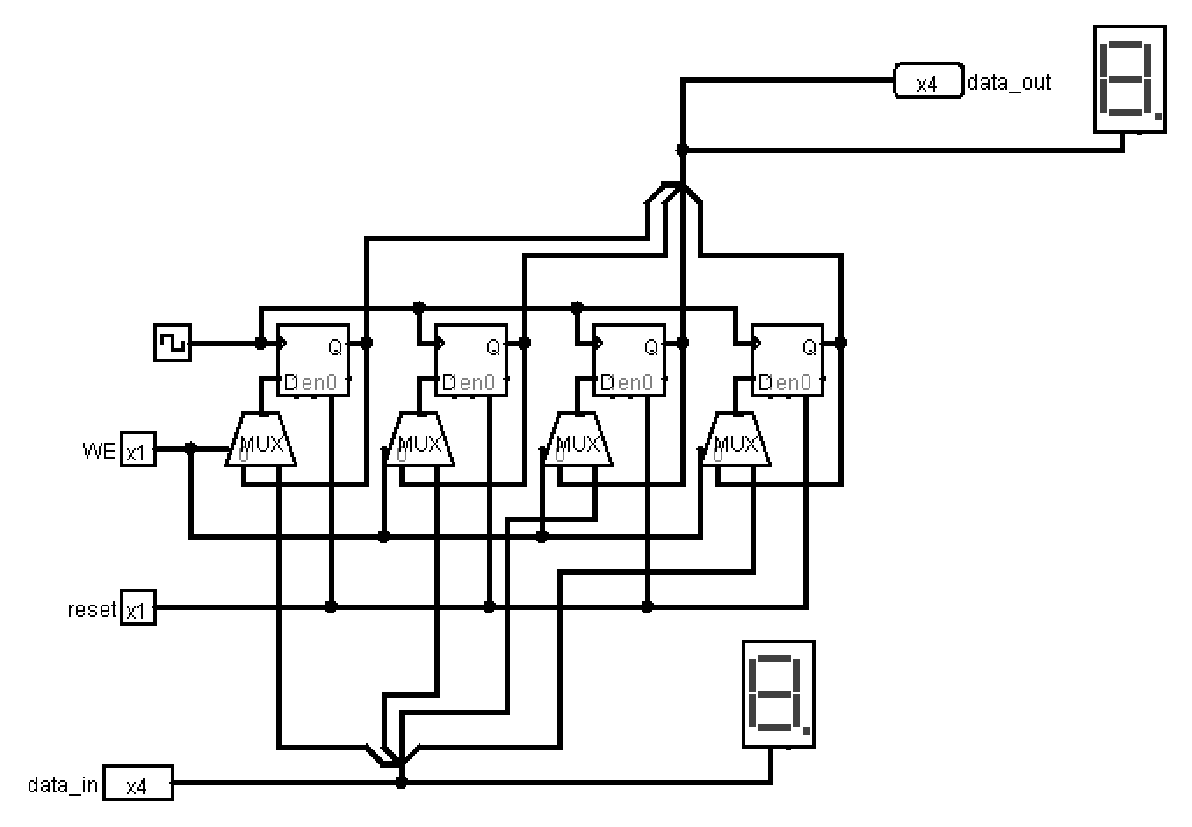
\includegraphics[width=0.75\columnwidth]{procesor/img/reg_4bit}%
\caption{Realizacija 4-bitnega registra v Logisimu z D-pomnilnimi celicami. Če so naslovni vhodi v multiplekserje aktivni (z drugimi besedami, če je $WE=1$), se stanje registra v naslednji urini periodi zamenja z vhodnim signalom \emph{data\_in}. V nasprotnem primeru se stanje registra ohranja.}%
\label{fig:reg_4bit}%
\end{center}
\end{figure}

\subsection{Programski števec}
Programski števec je v našem primeru posebna oblika registra s sledečima vhodoma:
\begin{itemize}
\item \emph{Reset}: ob aktivnosti vhoda se programski števec postavi na 0.
\item \emph{Inc} (Increment): če je vhod aktiven se vsebina programskega števca ob urini fronti poveča za 1 na način 0,1,2,3,0,1... 
\end{itemize}
Vsebino registra lahko beremo preko izhoda \emph{Address}, ki služi kot naslov za branje ukaza iz ukaznega pomnilnika. Realizacija programskega števca v Logisimu je prikazana na sliki \ref{fig:pc}.

\begin{figure}
\begin{center}
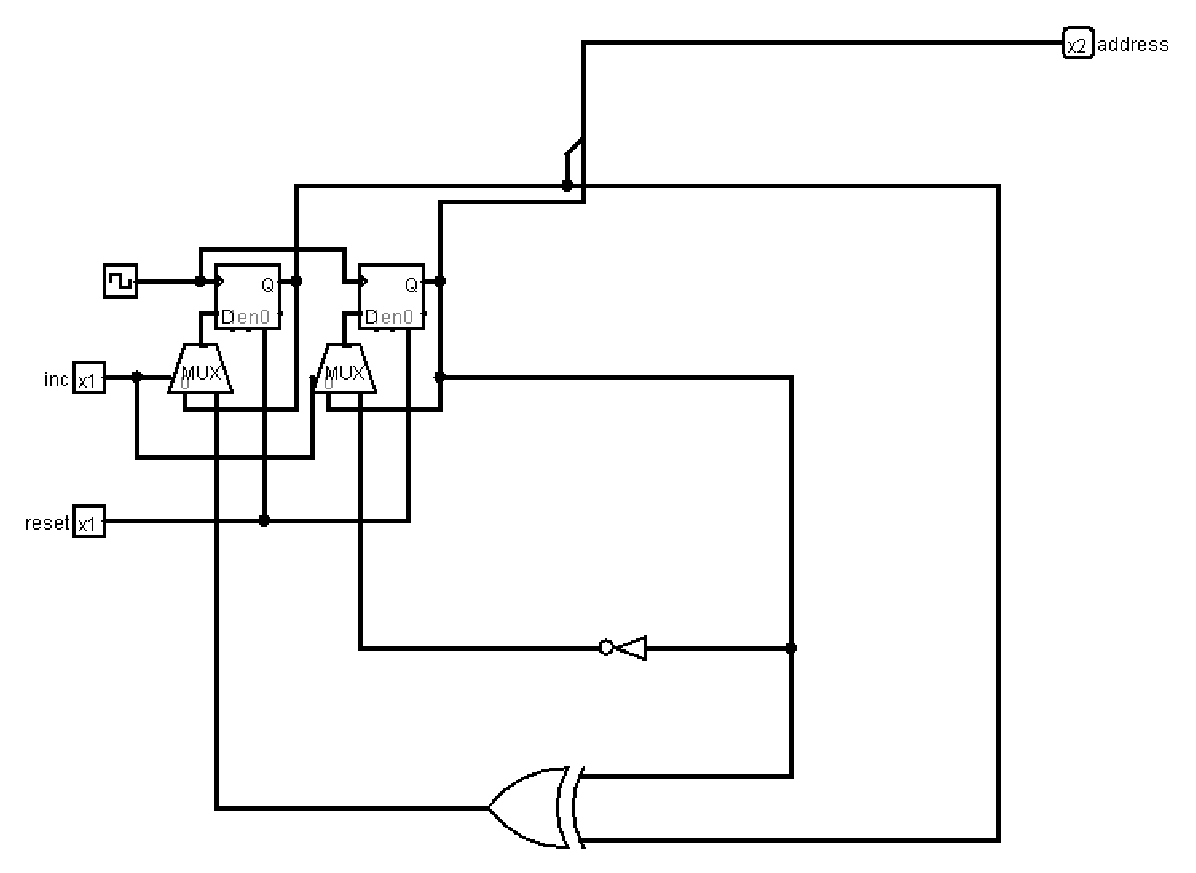
\includegraphics[width=0.75\columnwidth]{procesor/img/PC}%
\caption{Realizacija 2-bitnega programskega števca v Logisimu. Del kombinatorne logike ($XOR$ vrata in negator) predstavlja realizacijo povečanja vsebine programskega števca za 1. Če sta naslovna vhoda v multiplekserja ($inc$) aktivna, se stanje števca v naslednji urini periodi poveča. Če nista aktivna, se stanje ohranja.}%
\label{fig:pc}%
\end{center}
\end{figure}

\subsection{Seštevalnik}
Seštevalnik omogoča seštevanje dveh števil in je del aritmetično logične enote. V našem primeru imamo seštevalnik, ki sešteje dve 2-bitni števili. 2-bitni seštevalnik realiziramo z vezavo dveh 1-bitnih polnih seštevalnikov. Realizacija 1-bitnega polnega seštevalnika v Logisimu je prikazana na sliki \ref{fig:add_1bit}. Rezultat seštevanja dveh 1-bitnih števil $a$ in $b$ in prenosa \emph{carry\_in} gre na izhod $sum$. Izhod \emph{carry\_out} predstavlja prenos pri seštevanju.

\begin{figure}
\begin{center}
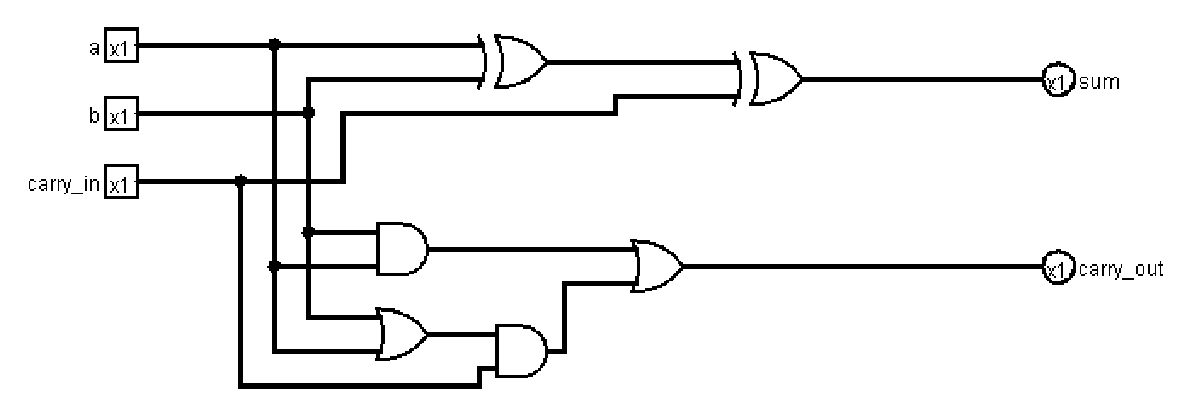
\includegraphics[width=0.75\columnwidth]{procesor/img/add_1bit}%
\caption{Realizacija 1-bitnega polnega seštevalnika v Logisimu.}%
\label{fig:add_1bit}%
\end{center}
\end{figure}

2-bitni seštevalnik lahko realiziramo z vezavo dveh 1-bitnih polnih seštevalnikov kot prikazuje slika \ref{fig:add_2bit}. Prenos pri seštevanju prvega seštevalnik (\emph{carry\_out}) uporabimo kot \emph{carry\_in} vhod v drugi seštevalnik.

\begin{figure}
\begin{center}
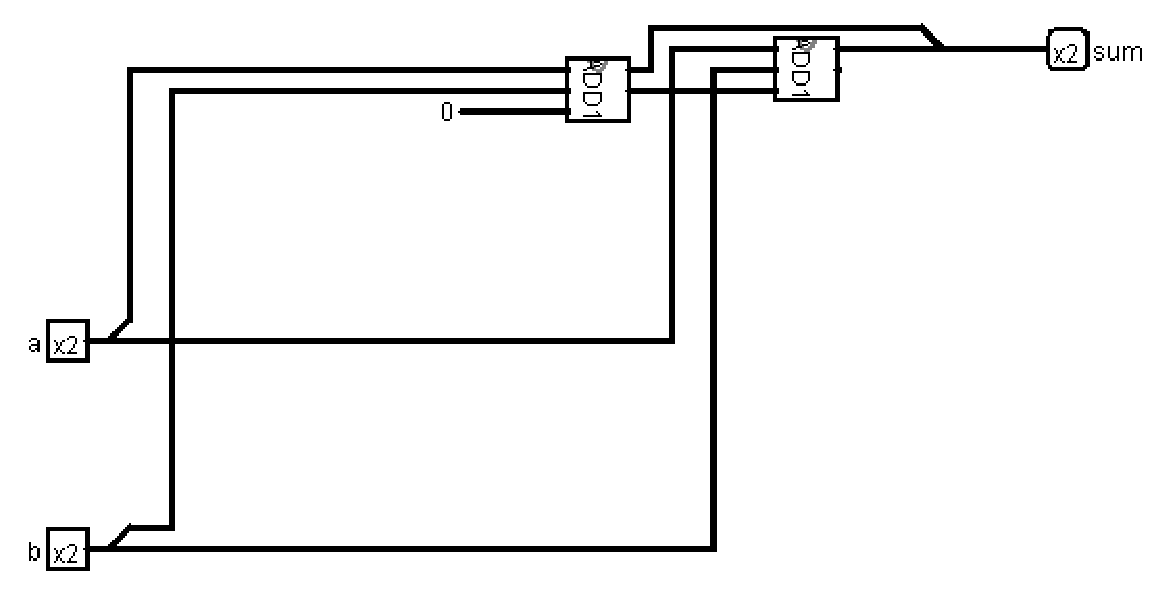
\includegraphics[width=0.75\columnwidth]{procesor/img/add_2bit}%
\caption{Realizacija 2-bitnega seštevalnika v Logisimu. Modula $ADD1$ predstavljata 1-bitna polna seštevalnika.}%
\label{fig:add_2bit}%
\end{center}
\end{figure}

\subsection{Odštevalnik}
\label{sec:odstevalnik}
Ker velja, da je odštevanje enako prištevanju negativnega števila ($a-b=a+(-b)$), lahko pri realizaciji odštevalnika uporabimo seštevalnik, pri čemer seštevamo števili $a$ in $-b$. V ta namen, moramo realizirati vezje, ki izračuna negativno vrednost števila $b$. Negativno vrednost dobimo s t.i. \emph{dvojiškim komplementom}, ki ga lahko izračunamo z uporabo sledeče enačbe
$$
- b = \ol{b} + 1
$$
Vezje za izračun dvojiškega komplementa prikazuje slika \ref{fig:complement}.
\begin{figure}
\begin{center}
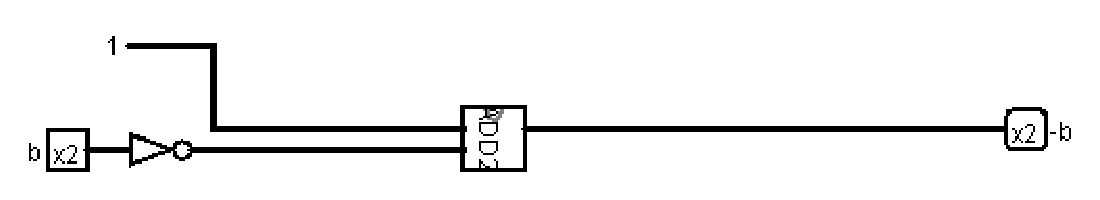
\includegraphics[width=0.75\columnwidth]{procesor/img/complement}%
\caption{Realizacija vezja za izračun dvojiškega komplementa v Logisimu. Modul $ADD2$ predstavlja 2-bitni seštevalnik. Dvojiški komplement izračunamo tako, da negirani vrednosti vhodnega signala $b$ prištejemo 1.}%
\label{fig:complement}%
\end{center}
\end{figure}

\subsection{Read Only Memory (ROM)}
ROM pomnilnik je pomnilnik iz katerega lahko programsko zgolj beremo. V našem primeru vanj pred začetkom izvajanja ročno zapišemo program. 

Vsebino ROM pomnilnika beremo tako, da na vhod \emph{A} ($Address$) pripeljemo naslovni signal. Na izhodu \emph{D} ($Data$) dobimo podatek, ki je zapisan na naslovu \emph{A}. Z $n$-bitnim naslovom lahko naslavljamo $2^n$ lokacij. 

V Logisimu mora biti pomnilnik za uporabo omogočen. Omogočimo ga tako, da na \emph{sel} ($Select$) vhod pripeljemo konstanto 1. 

\subsection{Random Access Memory (RAM)}
RAM pomnilnik je pomnilnik v katerega lahko tako pišemo kot tudi beremo. Pri pisanju v pomnilnik podamo podatek, ki ga želimo zapisati in naslov, na katerega želimo pisati. Pri branju iz pomnilnika podamo naslov, iz katerega beremo.

Pri uporabi RAM pomnilnika v Logisimu moramo upoštevati sledeče vhode:
\begin{itemize}
\item \emph{A} ($Address$): naslov iz katerega beremo oziroma na katerega pišemo. Z $n$-bitnim naslovom lahko naslavljamo $2^n$ lokacij.
\item \emph{D} ($Data\ in$): podatek, ki ga zapisujemo v pomnilnik.
\item \emph{str} ($Store$): podatek na vhodu \emph{D} se shrani v pomnilnik ob fronti ure, če je aktiven vhod \emph{str}.
\item \emph{sel} ($Select$): pomnilnik omogočimo tako, da na \emph{sel} vhod pripeljemo konstanto 1.
\item \emph{ld} ($Load$): podatek na naslovu \emph{A} gre na izhod pomnilnika $D$ ($Data\ out$) ob fronti ure samo, če je aktiven vhod \emph{ld}.
\end{itemize}
Iz pomnilnika beremo preko izhoda \emph{D} ($Data\ out$), tako da aktiviramo vhodni signal \emph{ld}. Podatek se pojavi na izhodu ob fronti ure.

\section{Realizacija opisanega procesorja}
Z ustrezno vezavo opisanih komponent lahko v Logisimu realiziramo preprost procesor.

Realizacijo opisanega procesorja v Logisimu prikazuje slika \ref{fig:procesor}.

\begin{figure}
\begin{center}
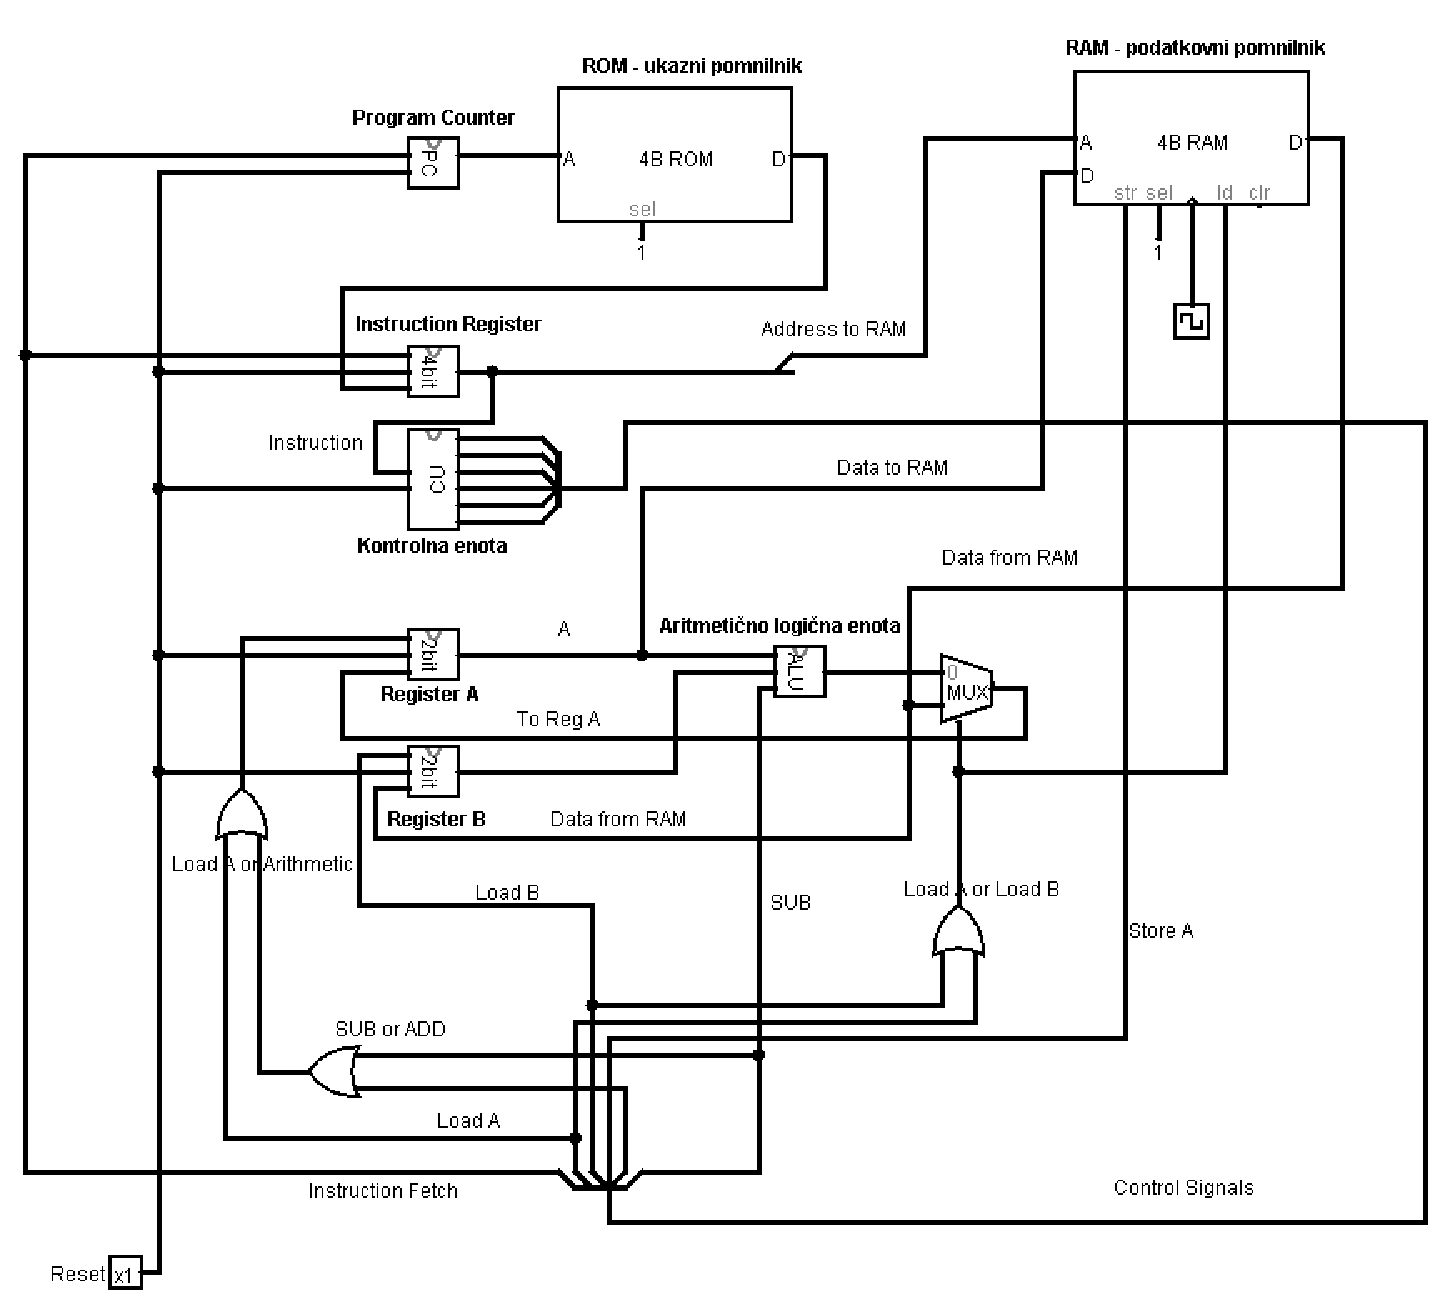
\includegraphics[width=0.75\columnwidth]{procesor/img/procesor}%
\caption{Realizacija preprostega procesorja v Logisimu.}%
\label{fig:procesor}%
\end{center}
\end{figure}


\section{Zgled delovanja procesorja}
\begin{zgled}
V ukazni pomnilnik procesorja v Logisimu bomo zapisali program, ki sešteje števili, ki sta zapisani na pomnilniških naslovih 0 in 1 podatkovnega pomnilnika in rezultat zapiše na pomnilniški naslov 2.

Najprej bomo program zapisali s t.i. mnemoniki:
\begin{alltt}
Load A 0
Load B 1
Add
Store A 2
\end{alltt}

S pomočjo tabele \ref{tab:ukazi} lahko ukaze zapišemo v dvojiški obliki:
\begin{alltt}
0000
0101
1100
1010
\end{alltt}

Ukaze vnesemo v ukazni pomnilnik (ROM) v šestnajstiški obliki:
\begin{alltt}
0
5
C
A
\end{alltt}

\end{zgled}
%\newpage

%\section*{Laboratorijske vaje}
%V ukazni pomnilnik procesorja realiziranega v Logisimu zapišite in preizkusite sekvenco ukazov (program), ki odšteje število zapisano na pomnilniškem naslovu 3 od števila zapisanega na pomnilniškem naslovu 2 in rezultat shrani na pomnilniški naslov 0.
%
%\bigskip
%\textbf{REŠITEV.}
%\bigskip
%
%Sekvenca ukazov (mnemonikov):
%\begin{alltt}
%Load A 2
%Load B 3
%Sub
%Store A 0
%\end{alltt}
%
%\bigskip
%
%Sekvenca ukazov v binarnem zapisu:
%\begin{alltt}
%0010
%0111
%1110
%1000
%\end{alltt}
%
%\bigskip
%
%Sekvenca ukazov v šestnajstiškem zapisu (kot jih zapišemo v ROM):
%\begin{alltt}
%2
%7
%E
%8
%\end{alltt}

